%!TEX root = ../Thesis.tex
\chapter{Spica rocket mission }
\textit{This chapter describes the rocket, elements of aerodynamics stability, the type of thrust vector control for the rocket, which is to be studied and controlled.  This is to understand what elements precede control and which influences are to be expected and what does the controller have to compensate for.}
\section{Spica rocket}
Spica is the next rocket developed and built by Copenhagen Suborbitals. The rocket aims to be the first crewed vehicle developed by the organisation and the first crewed amateur rocket in the world. Spica will be powered by a 100 kN liquid bi-propellant engine running on liquid oxygen and ethanol. Spica will have a diameter of 0.955 m, a total height of about 13 meters and a Gross Lift Off Weight of 4000 kg of which 2600 kg will be propellant.

From the Copenhagen Suborbitals website on Spica mission description: “Spica will be launched from an upgraded Sputnik platform capable of supporting the weight and space required. With a Gross Lift-Off Weight (GLOW) of 4000 kg and a thrust of 100 kN Spica will climb out with an initial Thrust To Weight Ratio (TTWR) of 2.55. 
At T+20 seconds it will go super sonic and at T+90 seconds the engine will shut off at a velocity of about 3600 km/h and an altitude of 50 km. 
From here Spica will coast to apogee at 105 km at T+190 seconds. A few seconds later the ballute will be deployed in order to stabilize the capsule through the thin part of the atmosphere. 
Approximately 9 minutes after launch at an altitude of 4 km the parachutes will unfold and provide a gentle landing in the Baltic Ocean where the recovery team will be ready to secure the capsule and the astronaut.”

\begin{figure}[h!]
  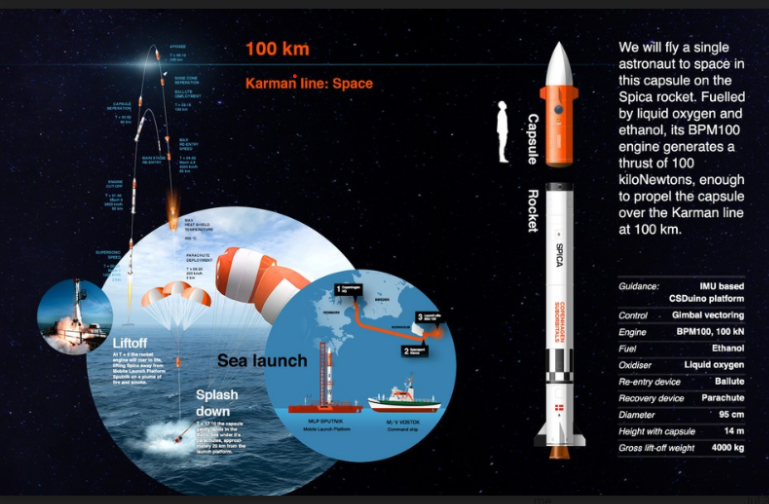
\includegraphics[scale=0.8]{graphics/Karman.png}
  \caption{Description of Spica rocket mission }
  \label{Spica mission}
\end{figure}

Rockets are launched from the military firing practice area ESD 139 in the Baltic Sea, 20 km east of the Danish island of Bornholm. It spans 70×35 km, and it is opened for launch by the Royal Danish Navy for the launch time window. 
The Danish and Swedish authorities close the airspace for air traffic in the hours prior to launch. The mission base is the seaside town Nexø on the east coast of Bornholm, also named ''Spaceport Nexø''. The launch platform is MLP-Sputnik, a metal platform powered by diesel engines. 

\begin{figure}[H]
  \centering
  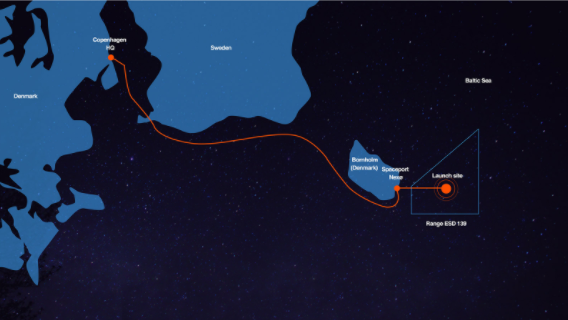
\includegraphics[scale=1]{graphics/launchsite.png}
  \caption{Rockets launch site in Baltic Sea}
  \label{launchsite}
\end{figure}

\section{Rocket aerodynamics and stability }

This section describes theoretical elements of rocket aerodynamics and aerial stability. The motivation is to fulfill the requirement of understanding elements affecting the flight significantly, preceding the control system design.
This section aims to answer the following questions: What affects rocket aerodynamic stability? What needs to be known before thrust vector control acts?

Flight stability is important for the vehicle in order to avoid tumbling, oscillations which cause extra drag and sloshing of the liquid propellants \cite{sutton2016rocket}. A primary concern is to prevent large-amplitude transient oscillations.
There are two components to stability: inherent stable design and active stabilisation from control systems. 
Inherent stability is specific to the rocket's design, that is, aerodynamic design meant to minimize drag. Such an example is the design of the nose cone and thrust alignment with body center of gravity. Fin stabilization is another important aspect of passive stability. 

\begin{figure}[h!]
  \centering
  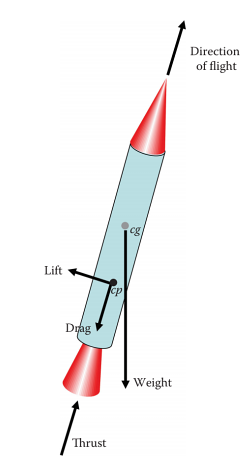
\includegraphics[scale=0.8]{graphics/forces.png}
  \caption{Forces acting on a rocket. Source: "Introduction to Rocket Science and Engineering" by : Travis Taylor, 2017}
  \label{forces}
\end{figure}

The aerodynamic forces acting on a rocket in flight are thrust, weight, lift and drag, dependant on the vehicle's shape, size, angle of attack.
Thrust and weight act on the rocket’s center of gravity (center of mass), while lift and drag forces act on the center of pressure. 
One of the main challenges in stabilizing a rocket comes from the shift in rocket's center of gravity as propellant is consumed during flight. This shift is more significant in large rockets, such as Spica, where the difference between  (Hobbs, 2010) \cite{hobbs2010basics}. It is necessary to know the absolute position of the two centers and the position relative to each other - their distance is termed stability margin. In order for the rocket to be stable in flight, the center of gravity needs to be above center of pressure \cite{taylor2017introduction}. 

\begin{figure}[h!]
  \centering
  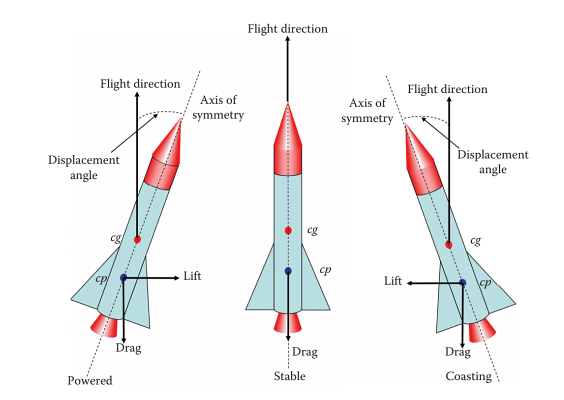
\includegraphics[scale=0.8]{graphics/flightAngle.png}
  \caption{Flight angle. Source: "Introduction to Rocket Science and Engineering" by : Travis Taylor, 2017}
  \label{forces}
\end{figure}

During powered flight, perturbations might occur which deviate the vehicle from its desired path, displacing its angle of attack. The aerodynamic forces will cause a torque about the center of gravity. During coasting (no engine thrust), the torque will be created in the opposite direction (Taylor, 2017). Having the proper stability margin, a rocket built top-heavy, allows the torques created by perturbations to self correct and stabilize the vehicle in flight - a phenomenon called restoring force. The restoring force is laminar flow of air occurring at high vehicle velocity. However, from launch and until achieving the necessary velocity, being top heavy, the rocket is highly unstable as it lifts off the launch rail \cite{taylor2017introduction}. It is not efficient to design a highly complex controller that can handle the large instability margins of the rocket launching right off the pad. 

The preferred approach is a controller that activates once the rocket is just off its rail, with enough velocity to take advantage of the restoring force stabilization and having its controller perform small adjustments.  To sum up, in flight, the rocket is subjected to disturbance torques which can be due to environmental torques, produced by the aerodynamic forces \cite{wertz2012spacecraft} or axial misalignments about the rocket’s center of mass.  
Passive stability is necessary but insufficient for large rockets, therefore active guidance and attitude control is necessary due to the inevitability of disruptions occurring in flight.
Active guidance and stabilization can be achieved by deflecting thrust so that a rotational effect is imparted to the body in flight. The chosen attitude control type  for Spica is thrust vector control through gimbaled engine. 

\begin{figure}[H]
  \centering
  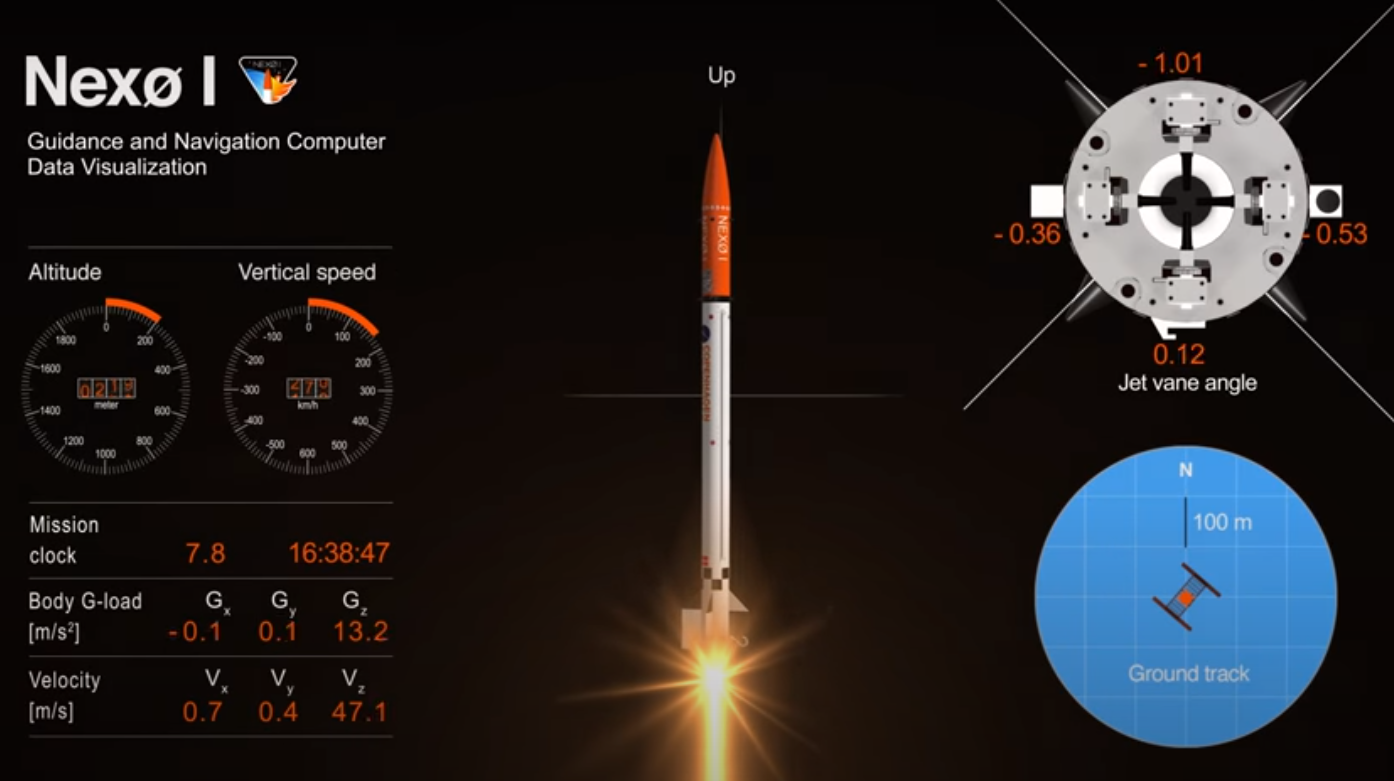
\includegraphics[scale=0.45]{graphics/Jetvanes.png}
  \caption{Capture of jet vanes function from a previous rocket}
  \label{jetvanes}
\end{figure}

\section{Thrust vector control}

\begin{figure}[H]
  \centering
  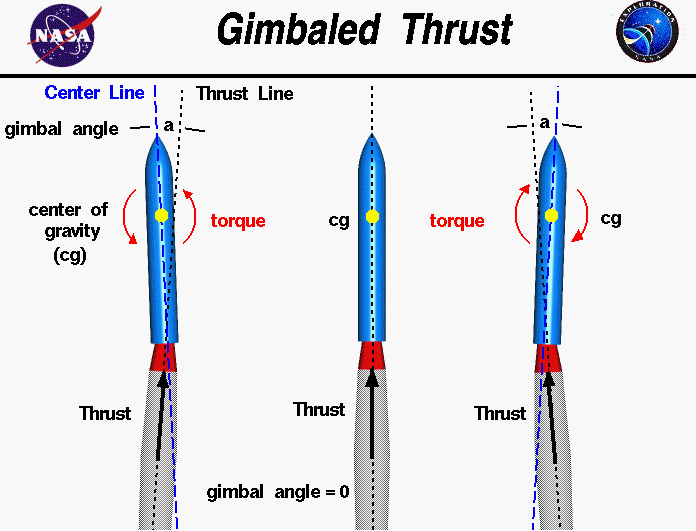
\includegraphics[scale=0.8]{graphics/gimbaled.png}
  \caption{Gimbaled thrust.  Source: NASA}
  \label{gimbaledthrust}
\end{figure}

All actively controlled Copenhagen Suborbitals rockets have featured jet vane based attitude and control systems. Jet vanes are made of graphite and allow deflection of the flow of the nozzle. While the system had great performance in previous rockets and insured stable control in flight, the next rocket cannot use jet vanes.
Due to their placement, jet vanes incur a drag (loss) of approximately 10 percent of the thrust - a significant loss for Spica-sized vehicles, which makes vanes not a feasible solution for this mission.
Graphite jet vanes are challenging to produce in Denmark, with the added difficulty of producing them in the size necessary for Spica.
Since jet vanes are not a suitable option for a Spica-sized rocket, there had to be a change towards another type of TVC. Out of the TVC types available for rockets, the organisation decided on gimbaled thrust.
Spica will be the first of Copenhagen Suborbitals rockets to feature a gimbal engine type of thrust vector control, as opposed to the previous solution of exhaust graphite vanes (jet vanes).

Spica will employ the more efficient gimbal system where the thrust chamber will be tilted, relative to the rocket’s center of gravity, to provide thrust vectoring and correct pitch and yaw. 
The advantages of the gimbal solution are that there will be no loss incurred due to drag as was the case in jet vanes, due to their placement. Another advantage is that the organisation is able to manufacture the gimbal system in-house. 
Since this is a major design change compared to the previous rockets the gimbal system will be tested on several unmanned flights prior to the first flight of crewed Spica.
The chosen TVC of gimbaled engine allows for four degrees of freedom, pitch and yaw control axes.
The roll control will be handled by a separate control system, out of the scope of this project - a reaction control system consisting of air thrusters. 
The TVC in this project will attempt to simulate gimbal working principles, that is, deflection of thrust in order to stabilize the rocket about its center of mass, with the difference of being tested in one axis.

\textit{This chapter introduced a summary of the technical and theoretical considerations preceding the work on navigation and control. Following content will address the building process of the prototype and its constituting elements.}


